\documentclass[
	letterpaper, % Paper size, specify a4paper (A4) or letterpaper (US letter)
	10pt, % Default font size, specify 10pt, 11pt or 12pt
]{CSUniSchoolLabReport}

%----------------------------------------------------------------------------------------
%	REPORT INFORMATION
%----------------------------------------------------------------------------------------

\title{Electrocardiogram\\ Circuits \& Signals \\ EECE2150} % Report title

\author{Michael \textsc{Brodskiy}}

\date{April 20, 2023} % Date of the report

%----------------------------------------------------------------------------------------


\begin{document}

\maketitle % Insert the title, author and date using the information specified above

\begin{center}
	\begin{tabular}{l r}
		Date Performed: & April 6, 2023 \\ % Date the experiment was performed
        Partner: & Juan \textsc{Zapata}, Oluwalaanu \textsc{Adeboye} \\ % Partner names
		Instructor: & Professor \textsc{Sun} % Instructor/supervisor
	\end{tabular}
\end{center}

\setcounter{section}{-1}

\section{Introduction}

The purpose of this laboratory experimentation was to unify all of the course concepts. Through integration of rudimentary circuit components like resistors, capacitors and inductors, in tandem with more complex components like operational amplifiers and band-pass filters, the goal was to construct a circuit that, when connected to three electrodes on the body, would generate a filtered electrocardiogram signal. Additionally, an analog-to-digital converter was then used to generate a heart rate plot from a sample.

\section{Discussion and Analysis}

\subsection{Part I}

\subsubsection{Q1} The signal is extremely noisy, but something resembling a heartbeat can somewhat be seen. The signal appears to be almost a solid block with slight, periodic, drops and peaks.

\subsection{Part II}

\subsubsection{Q2} If a low heart rate is 30 bpm $\rightarrow$ .5 bps $\rightarrow f_c=.5[\si{\hertz}]$ for the high pass; This means $f_c=\frac{1}{2\pi RC}=.5$, and, if $C=.1[\si{\micro\farad}]$, $R\approx300[\si{\kilo\ohm}]$. This makes the actual cutoff $.53[\si{\hertz}]$. In rad/s, the cutoff is $1.06\pi$. It was clear that a pass-band filter was necessary to create a well-filtered ECG. To remove the DC component, we removed anything below the $.53[\si{\hertz}]$ cutoff. A regular heartbeat can be as slow as $1[\si{\hertz}]$, so we mustn't filter it out. The gain for this filter is 3. If the in-band gain were too low, the signal would not be picked up by the oscilloscope. To high of a gain would oversaturate the filter and cut off the peaks that we are looking for.

\subsubsection{Q3} A 10$[\si{\hertz}]$ cutoff frequency for the low pass results in signal attenuation, and subsequently a difficulty in recognizing the signal (shown in Figure \ref{fig:1}). With 1000$[\si{\hertz}]$ (Figure \ref{fig:2}), practically nothing is filtered, and there is lots of noise. We chose the final frequency as 100$[\si{\hertz}]$, as it seemed like a good mid-ground between the two, and it turned out to work well.

\begin{figure}[H]
  \centering
  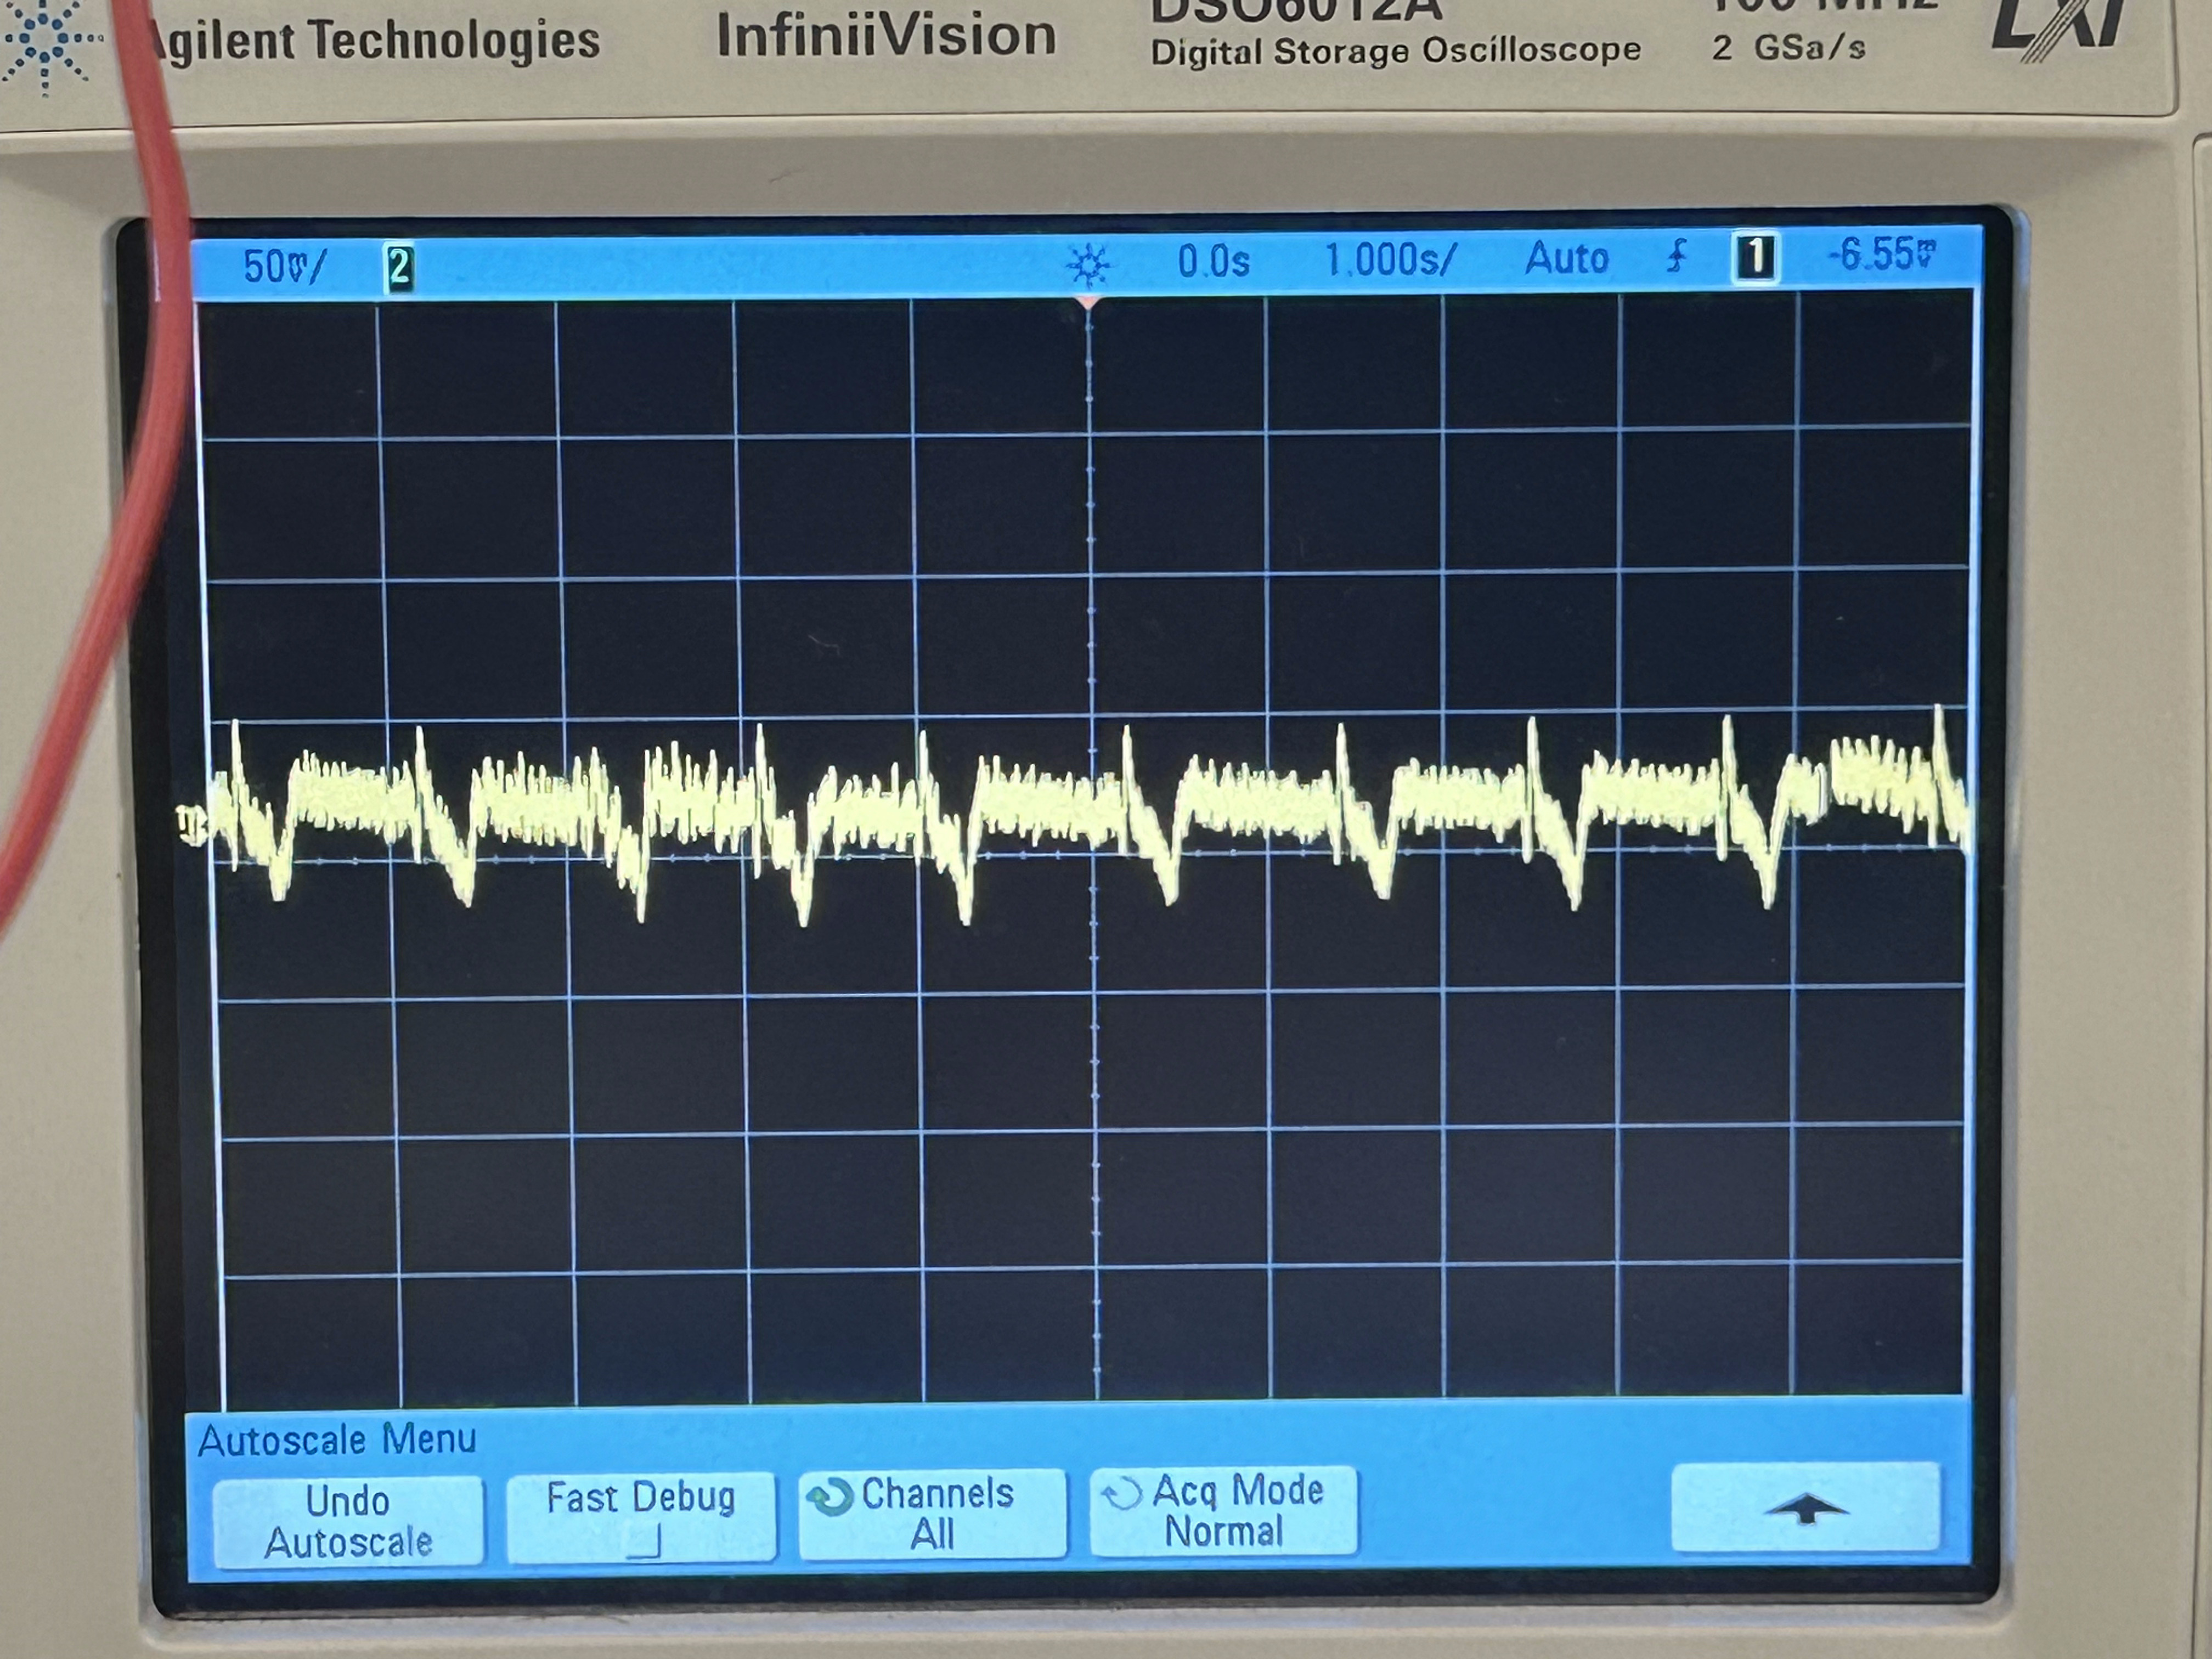
\includegraphics[width=.9\textwidth]{Figures/L15Q3.jpg}
  \caption{$10[\si{\hertz}]$ Cutoff}
  \label{fig:1}
\end{figure}

\begin{figure}[H]
  \centering
  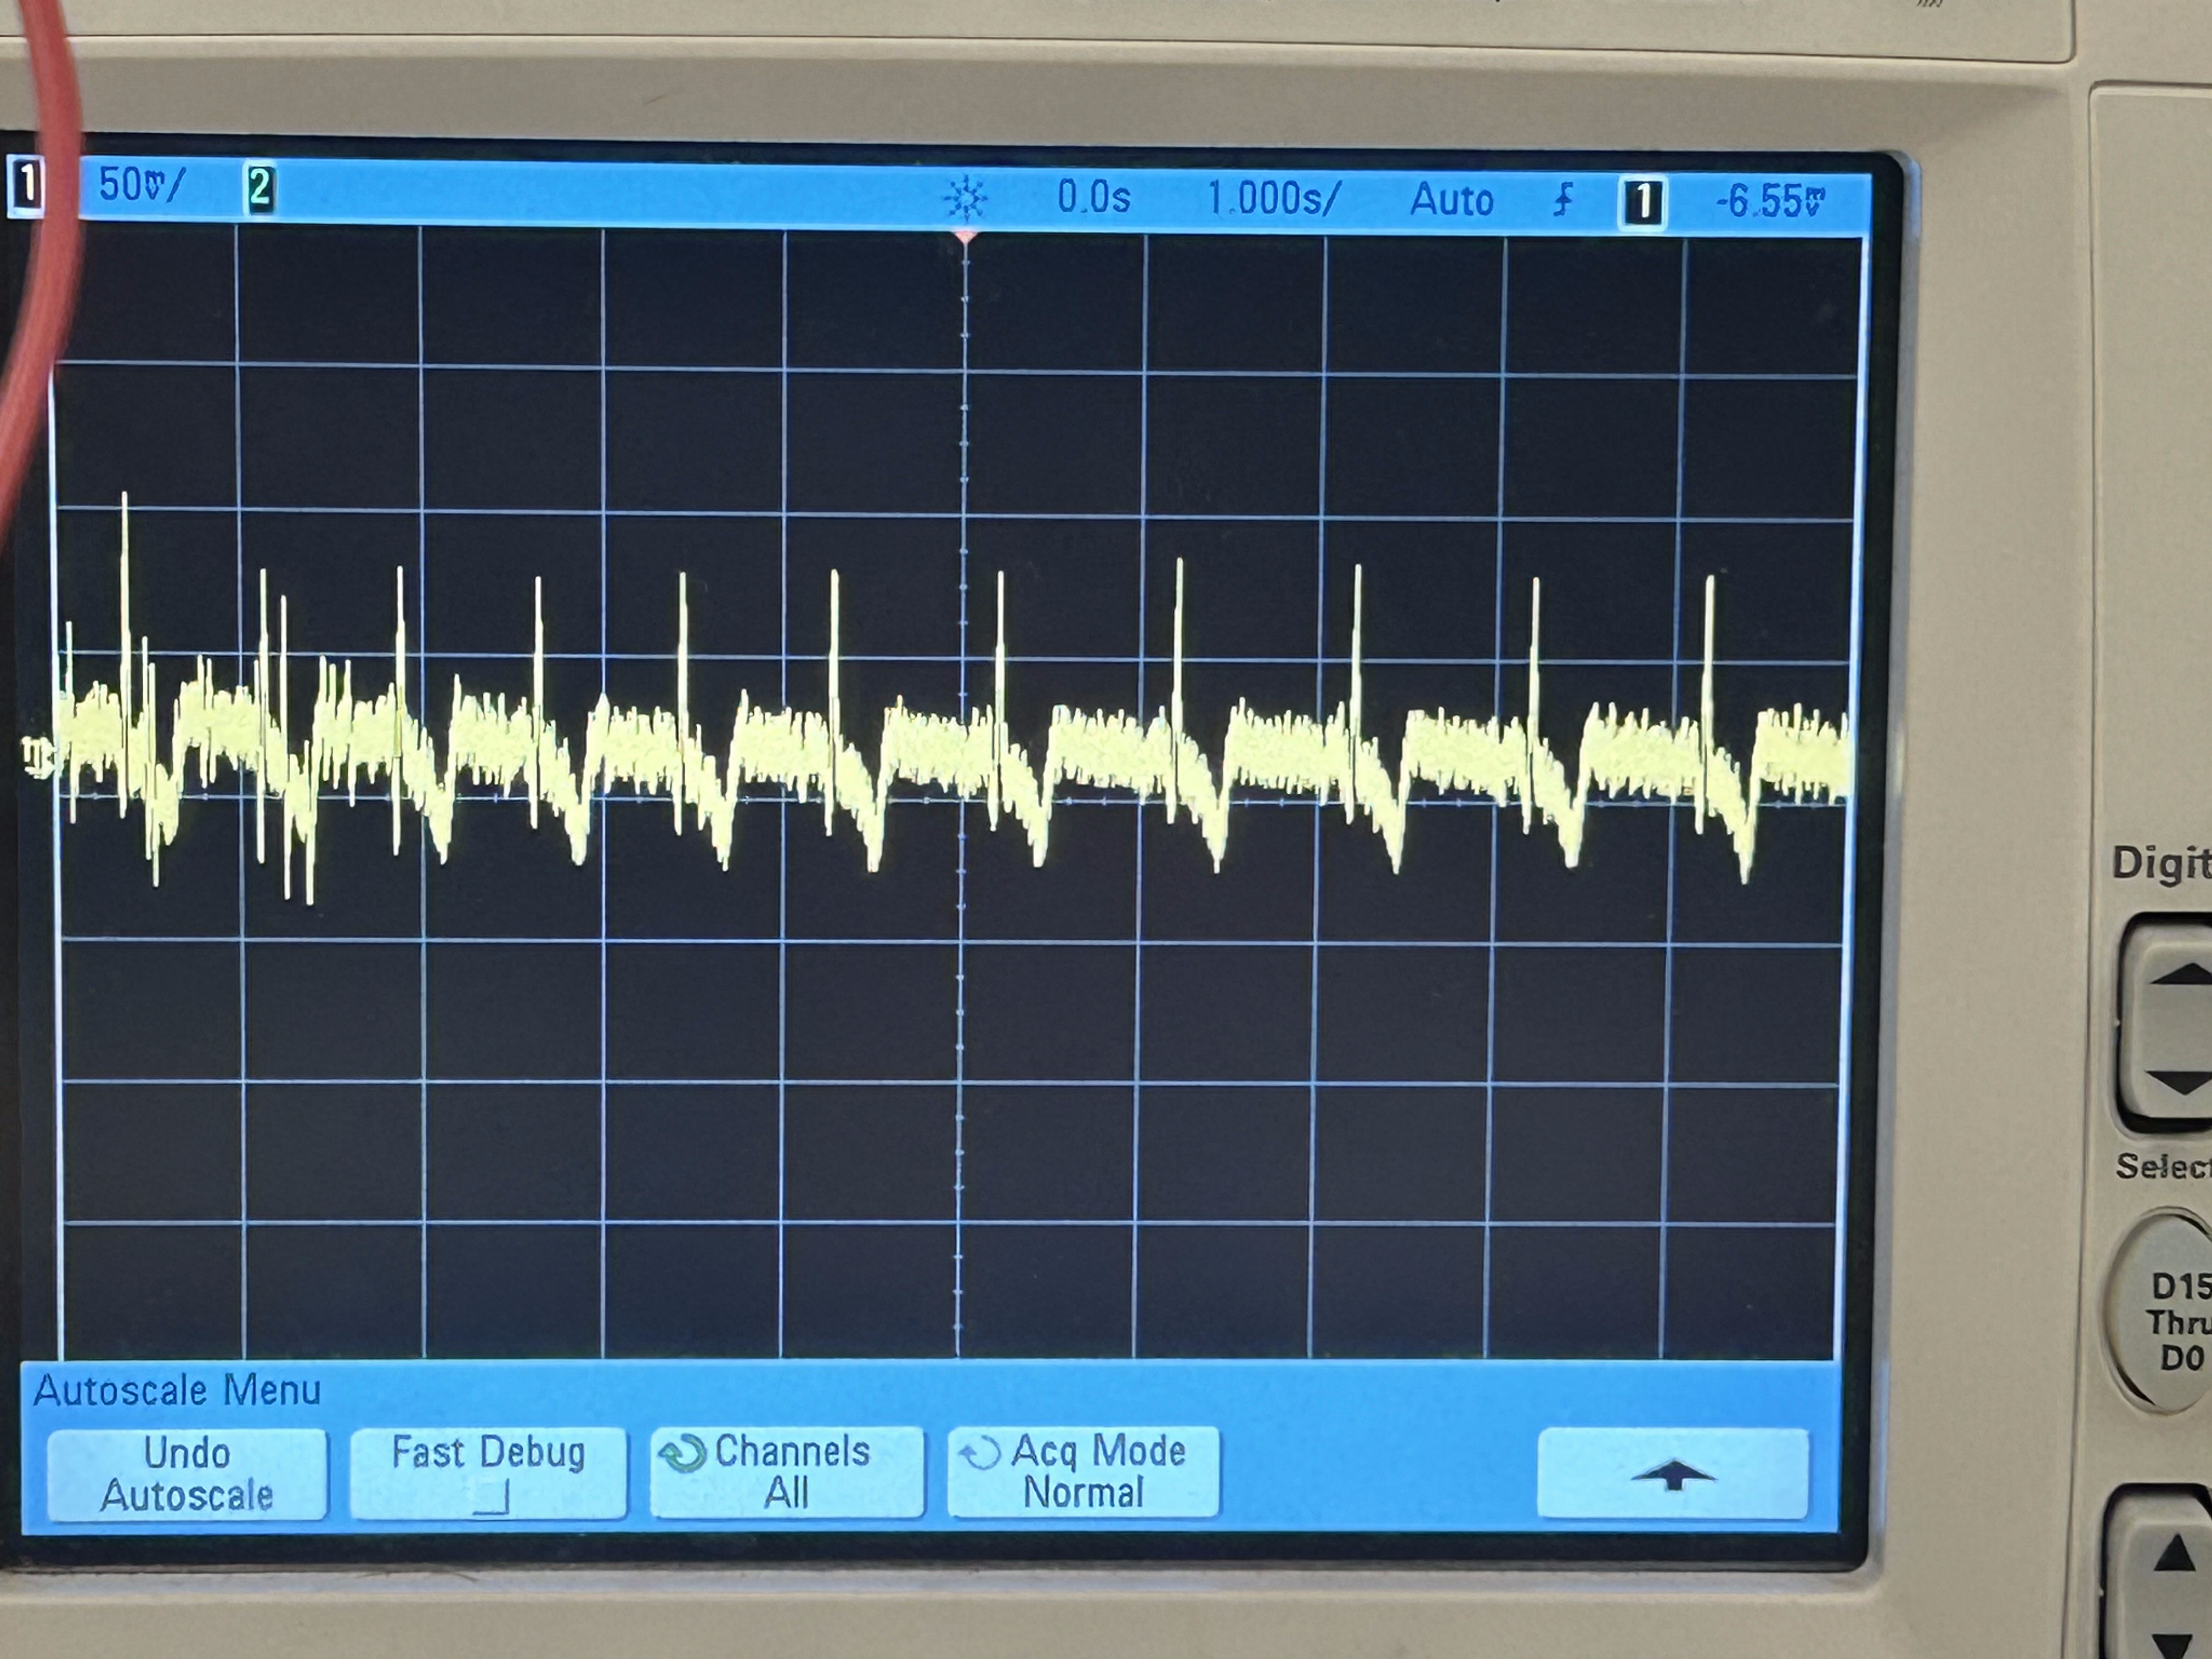
\includegraphics[width=.9\textwidth]{Figures/L15Q3-2.jpg}
  \caption{$1000[\si{\hertz}]$ Cutoff}
  \label{fig:2}
\end{figure}

\subsubsection{Q4} The final touches regarding the circuit mostly had to do with increasing the gain an adequate amount to use nearly the entire boundaries, without saturation. As the gains were adjusted across the operational amplifiers to generate the best signal, we were able to reach a peak of roughly $1.4[\si{\volt}]$ without saturating. The circuit is shown in Figures \ref{fig:3} and \ref{fig:4}

\begin{figure}[H]
  \centering
  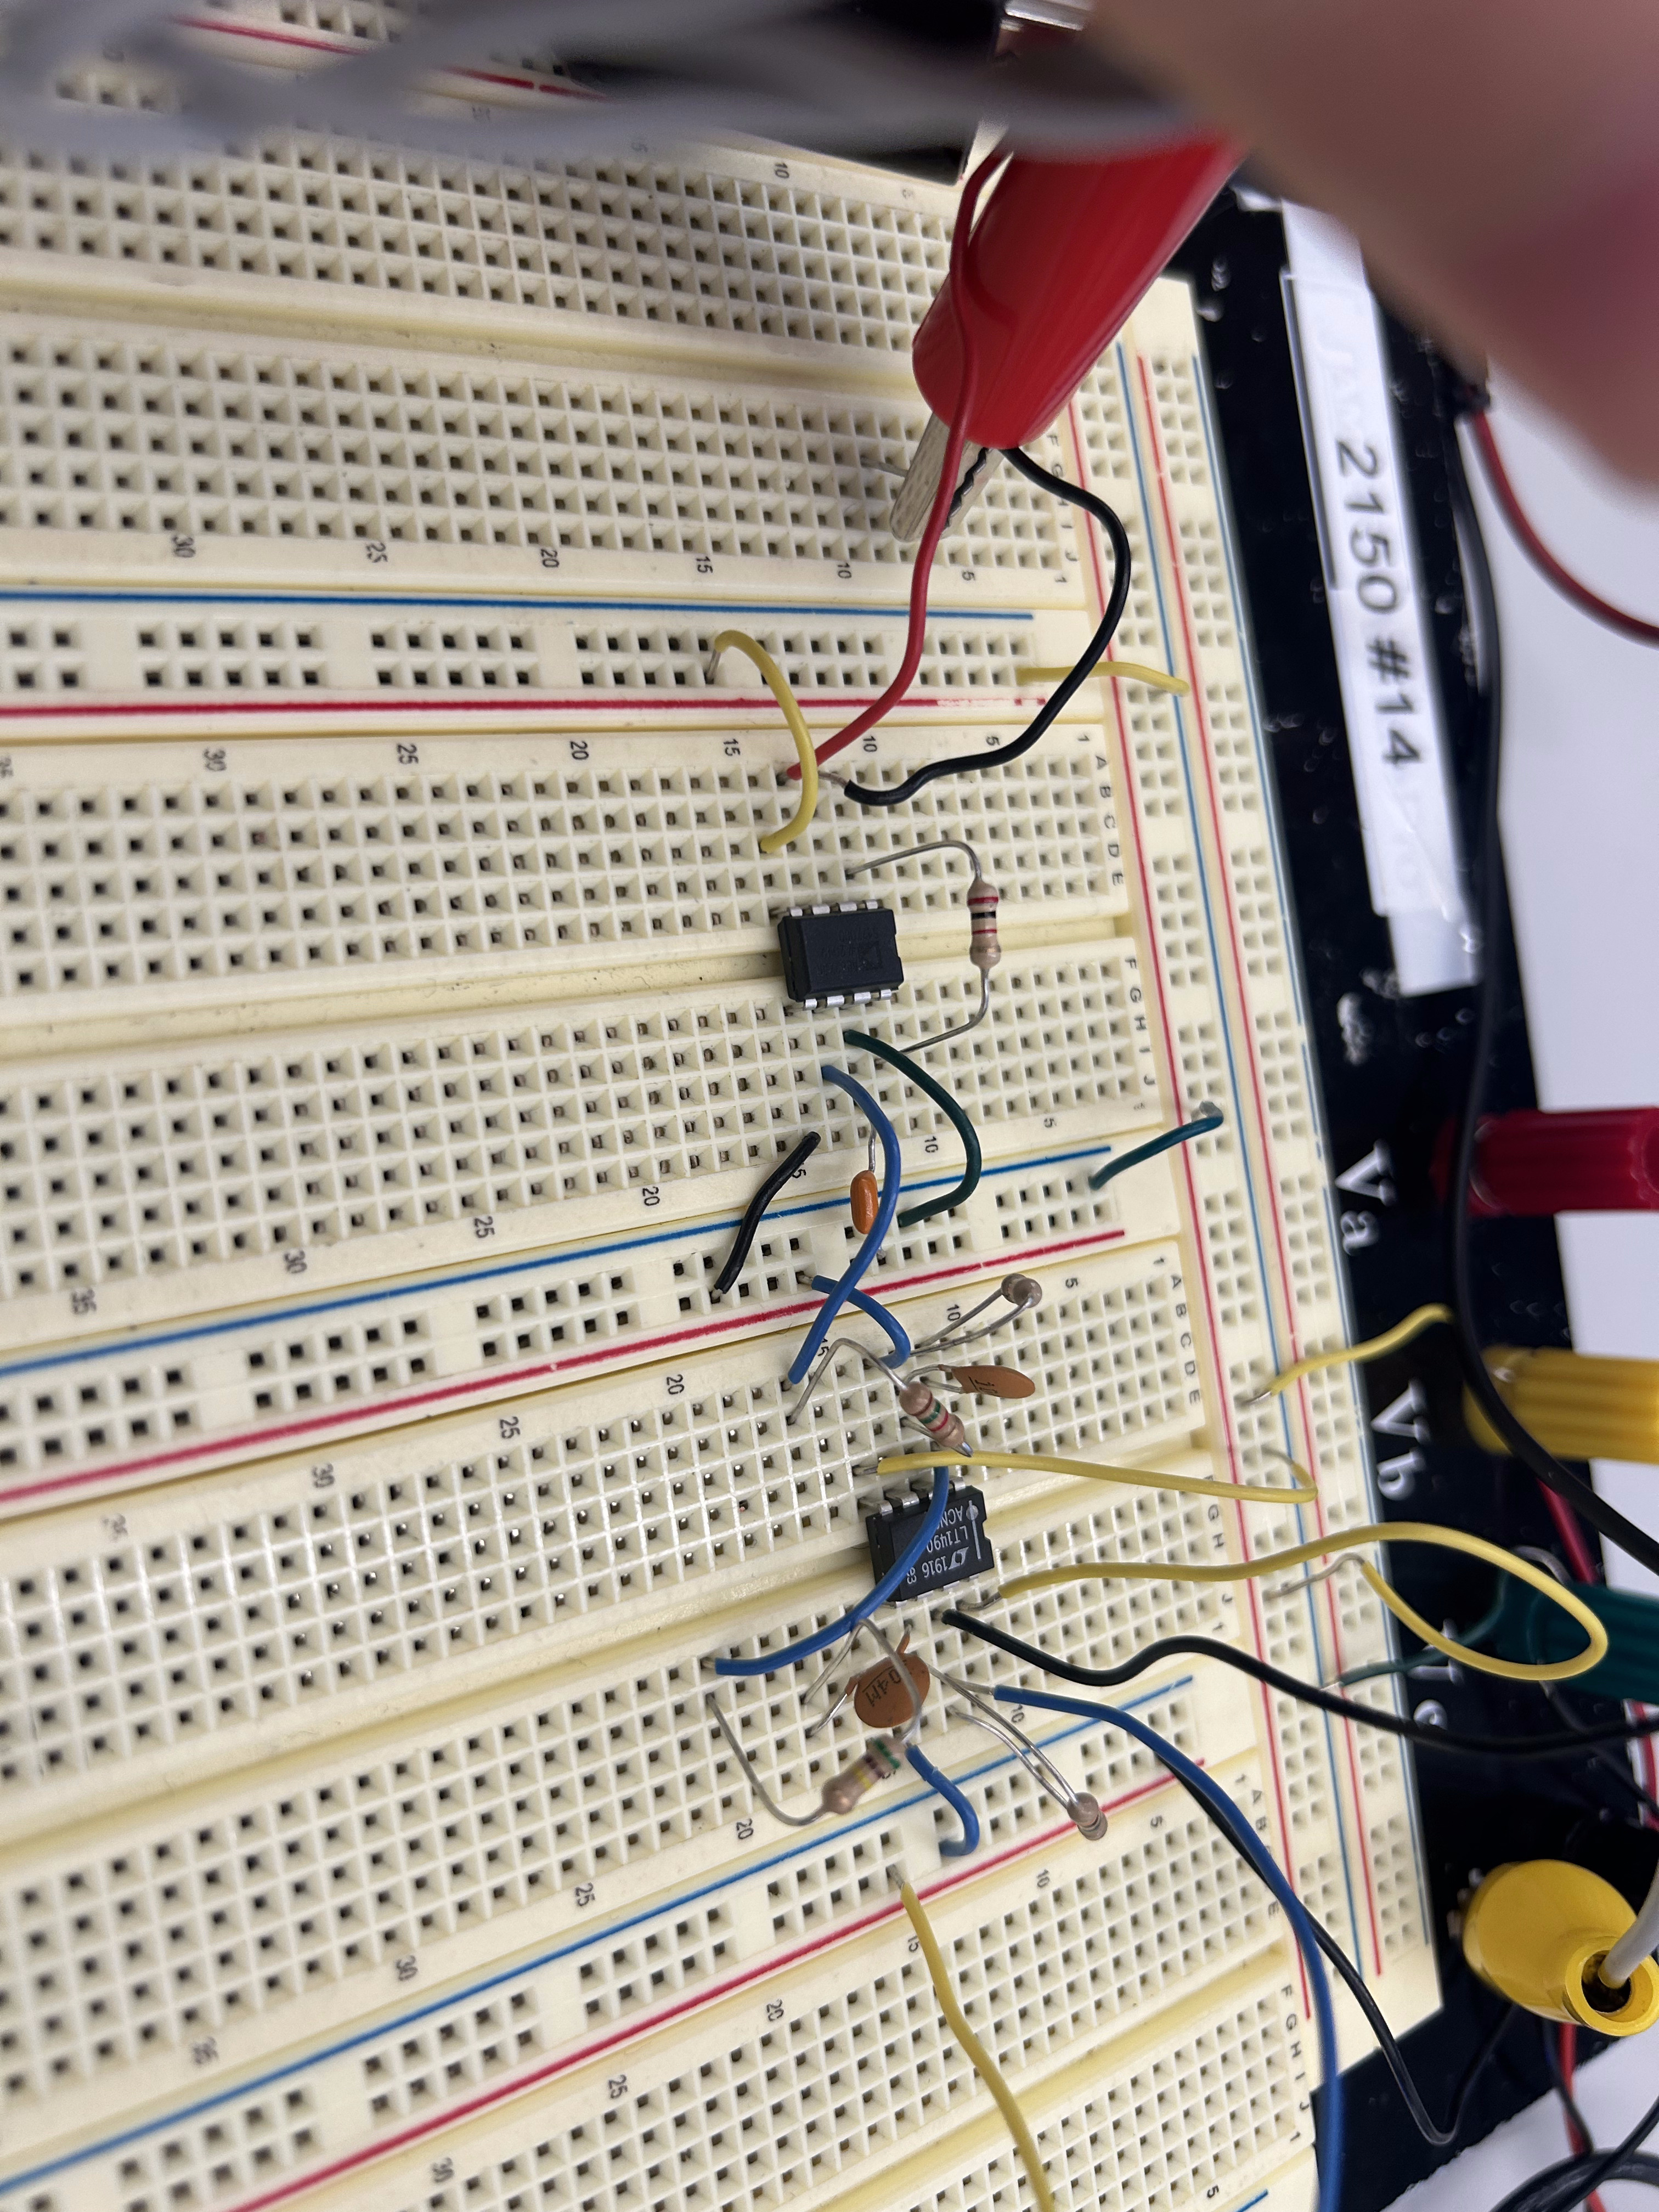
\includegraphics[width=.5\textwidth,angle=90]{Figures/L15Q4.jpg}
  \caption{Physical Circuit}
  \label{fig:3}
\end{figure}

\begin{figure}[H]
  \centering
  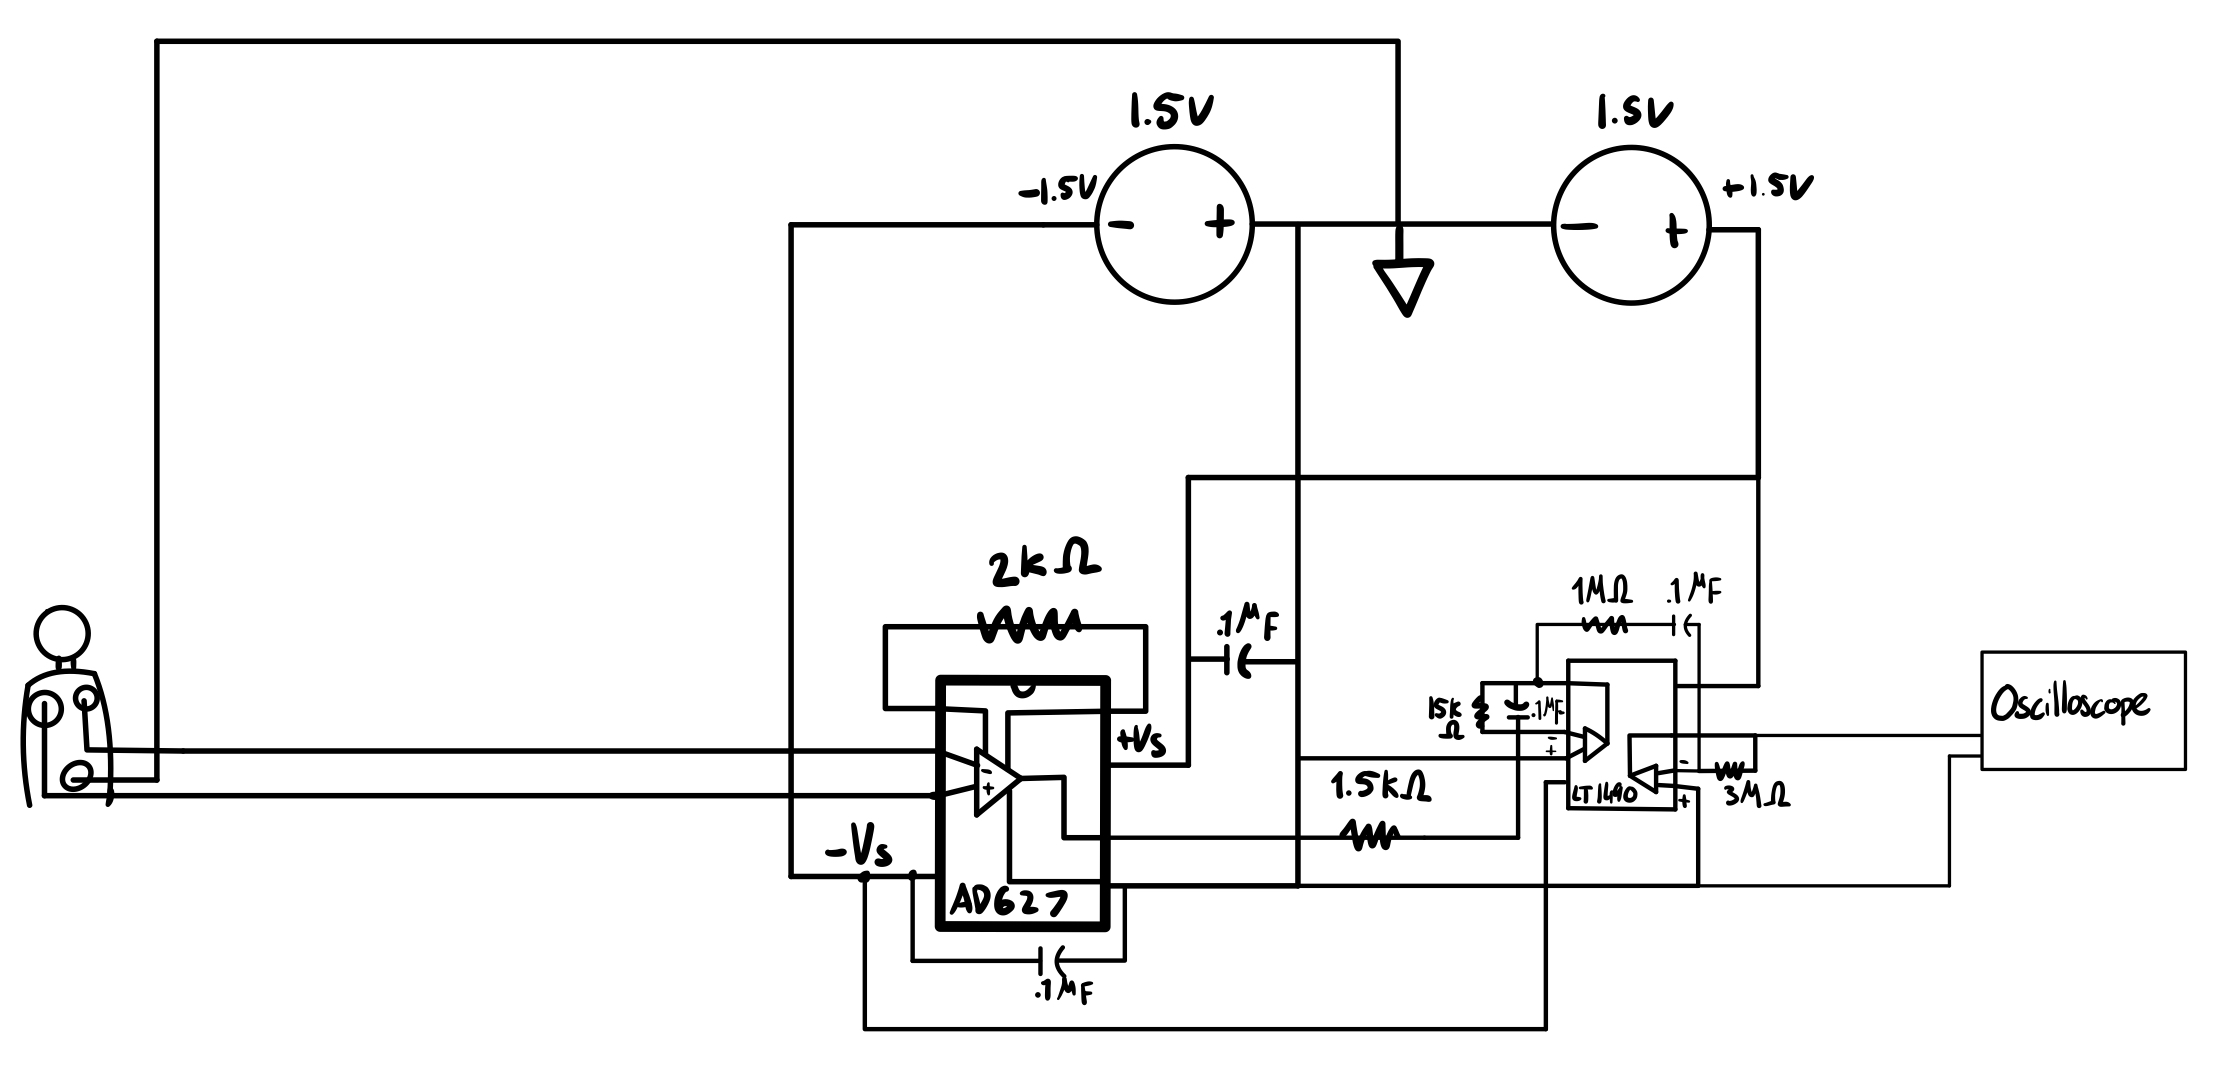
\includegraphics[width=.9\textwidth]{Figures/L15Q4-2.png}
  \caption{Circuit Diagram}
  \label{fig:4}
\end{figure}

\subsubsection{Q5} The plots generated through analog-to-digital conversion are shown in Figures \ref{fig:5} and \ref{fig:6} below.

\begin{figure}[H]
  \centering
  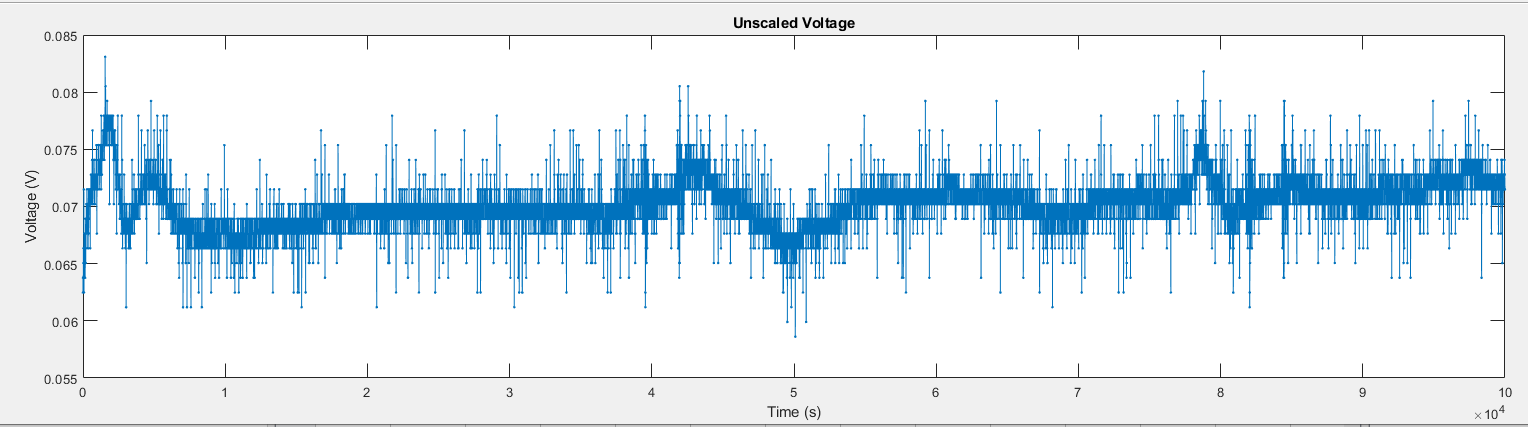
\includegraphics[width=.9\textwidth]{Figures/L15Q5.png}
  \caption{Unscaled Voltage Output}
  \label{fig:5}
\end{figure}

\begin{figure}[H]
  \centering
  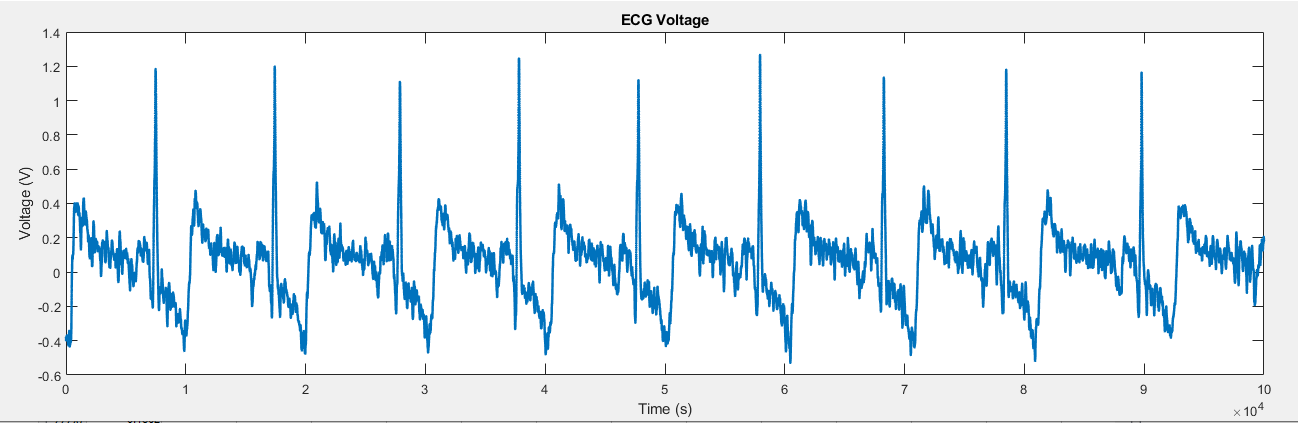
\includegraphics[width=.9\textwidth]{Figures/L15Q5-2.png}
  \caption{Scaled Voltage Output}
  \label{fig:6}
\end{figure}

The final, cleanest signal we attained is shown in Figure \ref{fig:7} below.

\begin{figure}[H]
  \centering
  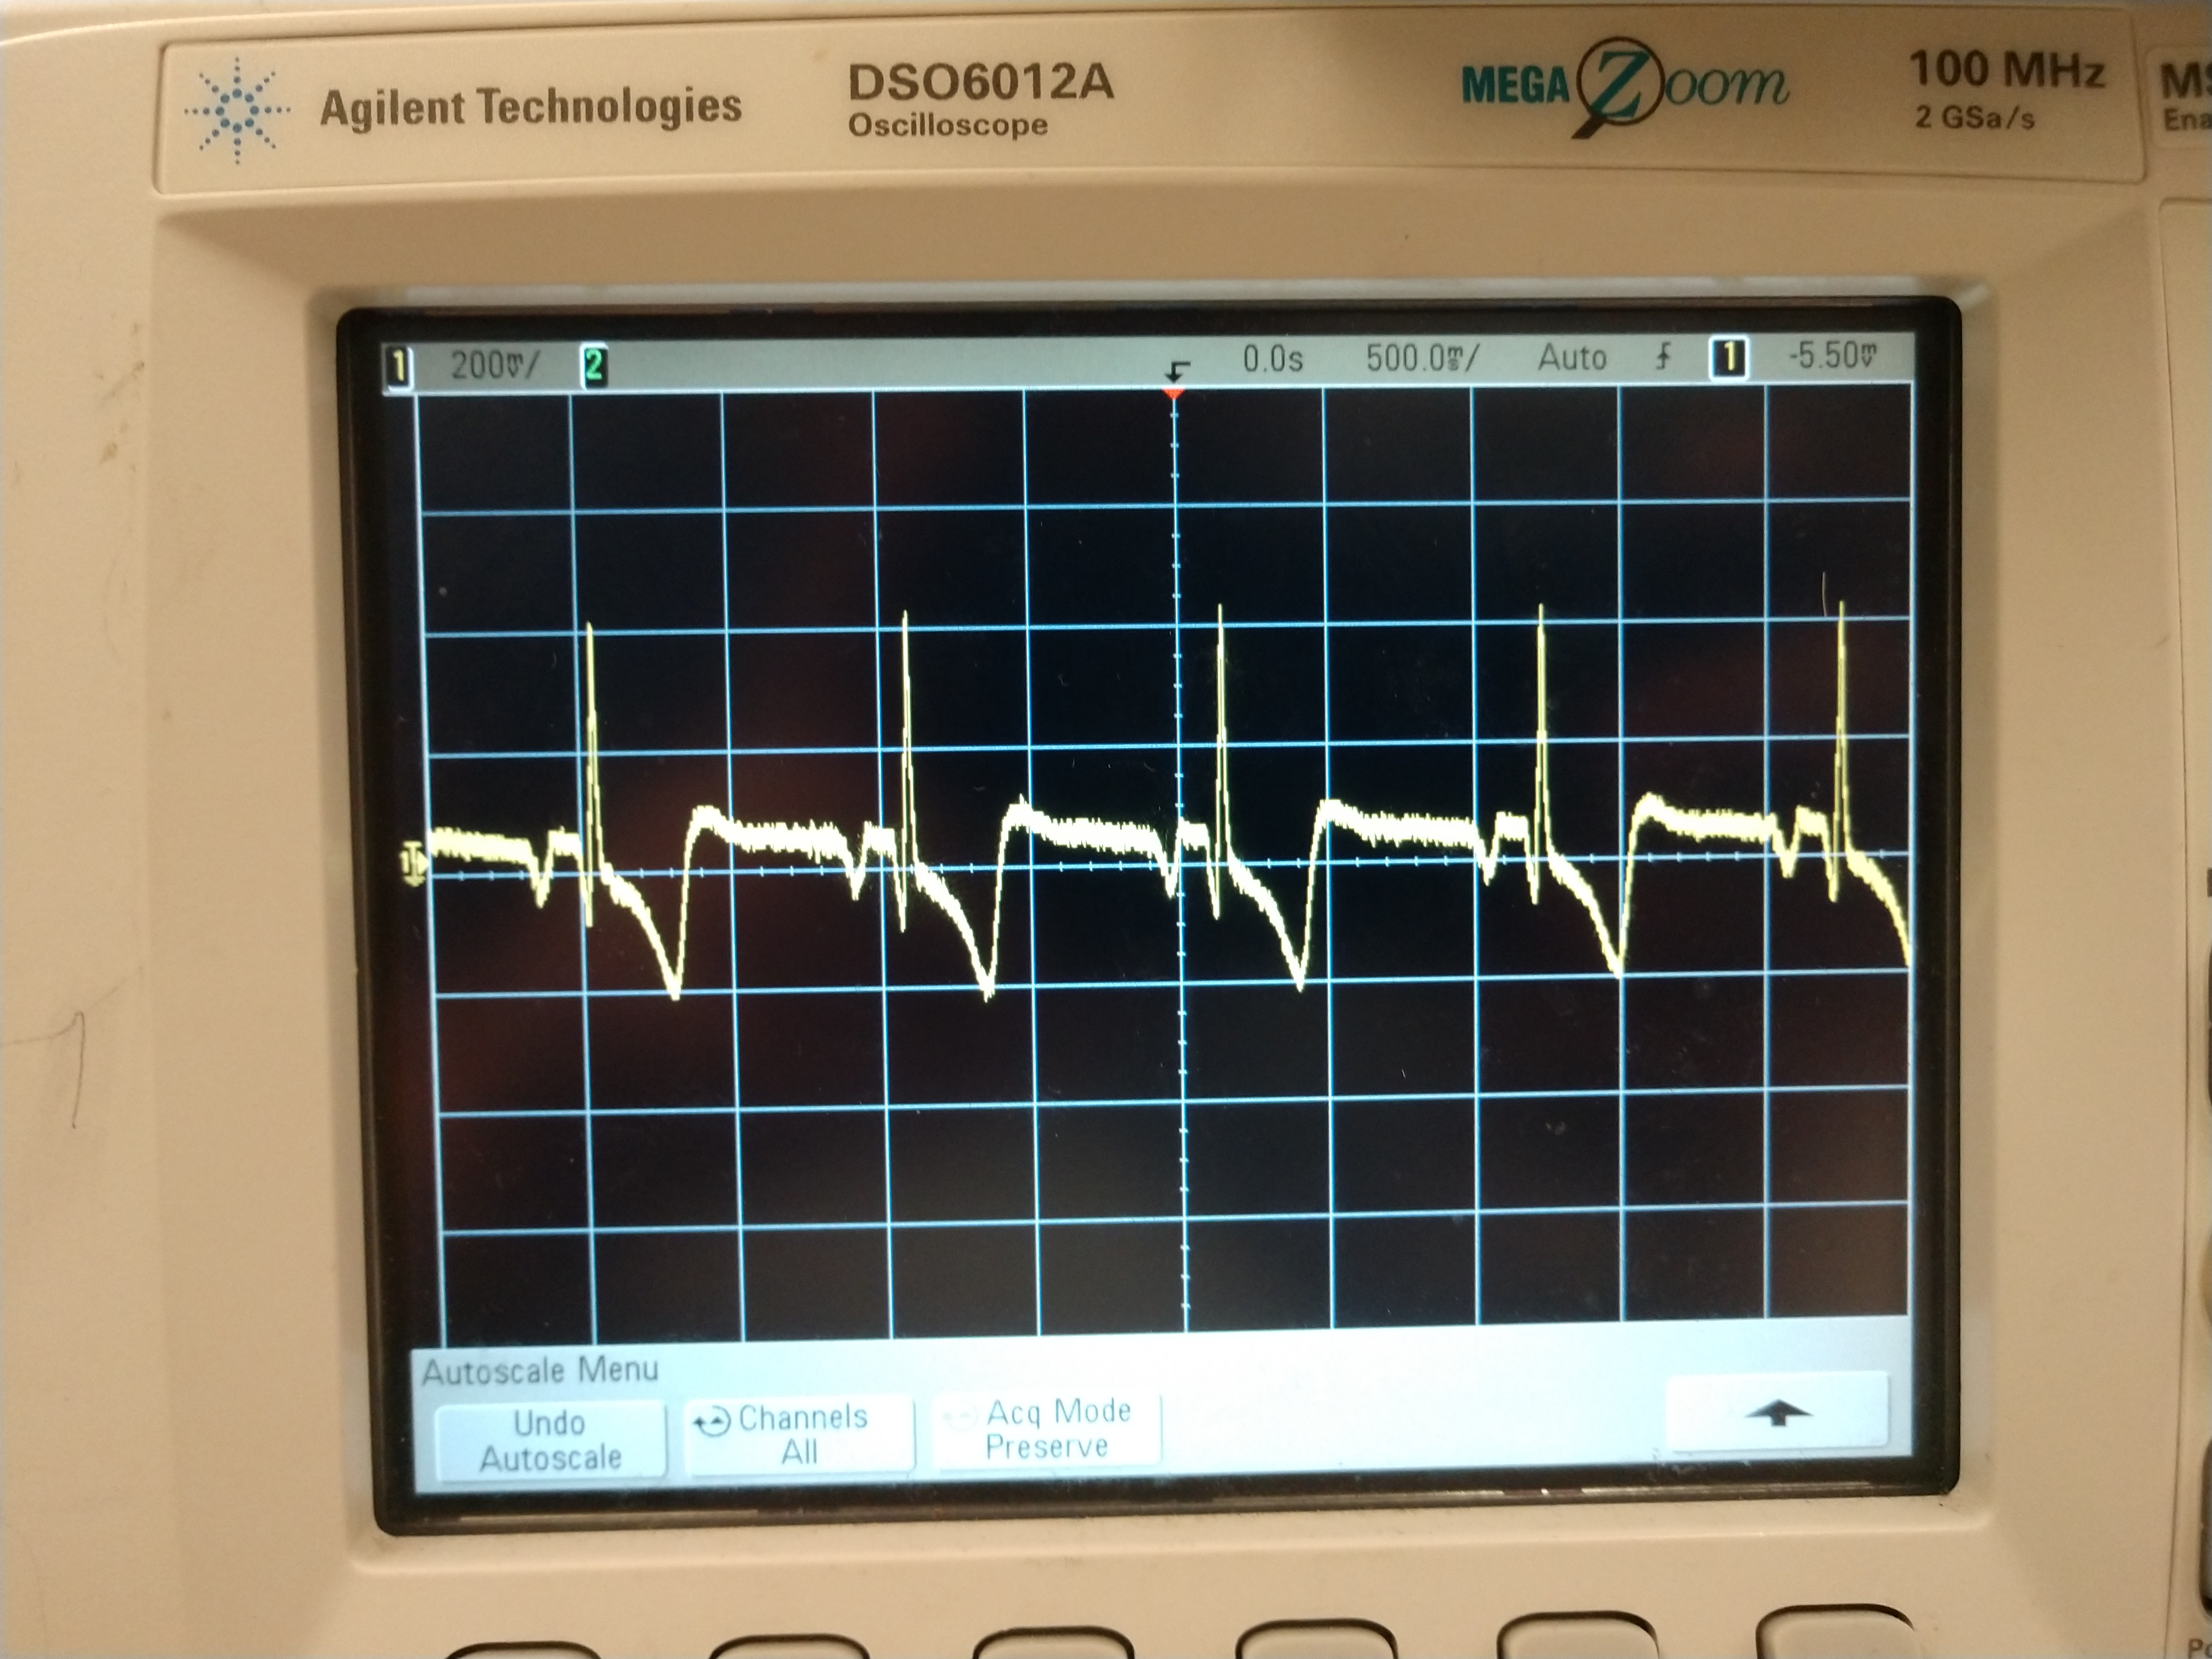
\includegraphics[width=.9\textwidth]{Figures/L15.jpg}
  \caption{Final Signal}
  \label{fig:7}
\end{figure}

\section{Conclusion}

Overall, this laboratory experiment allowed for an adequate unification of course concepts. By reiterating the basics and strengthening more advanced and, thus, difficult concepts, the lab creates a stronger understanding of all critical course concepts.

\end{document}
